\subsubsection{Subsystem Overview}

The Base Station is a mobile device that connects to the computing platform on the multirotor. In particular, it performs the following tasks:
\begin{itemize}
    \item Displays the status of the system
    \item Displays the ML results in real-time (by overlaying the results over live video)
    \item Remotely configures the computing platform (ex. starting object detection)
\end{itemize}

\subsubsection{Device Selection}
We considered two classes of devices which could be used as a base station: laptops and smart mobile devices (such as cellphones or tablets). The common features of these two options are: they are both equipped with a screen which can be used to display the video and ML results, they both have a Wi-Fi transceiver (\textbf{F.BS.3}), and they both have non-volatile storage which can be used to store results (\textbf{F.BS.6}).

To allow for the greatest cross-compatibility across potential client devices, the base station was designed to operate on a Node.js web-server framework. While this necessitates the use of a laptop computer to act as a centralized server, one may utilize additional (potentially more portable) devices to connect to the web application to view the results if desired.

\subsubsection{Functionality}

\begin{figure}[H]
\begin{mdframed}
\centering
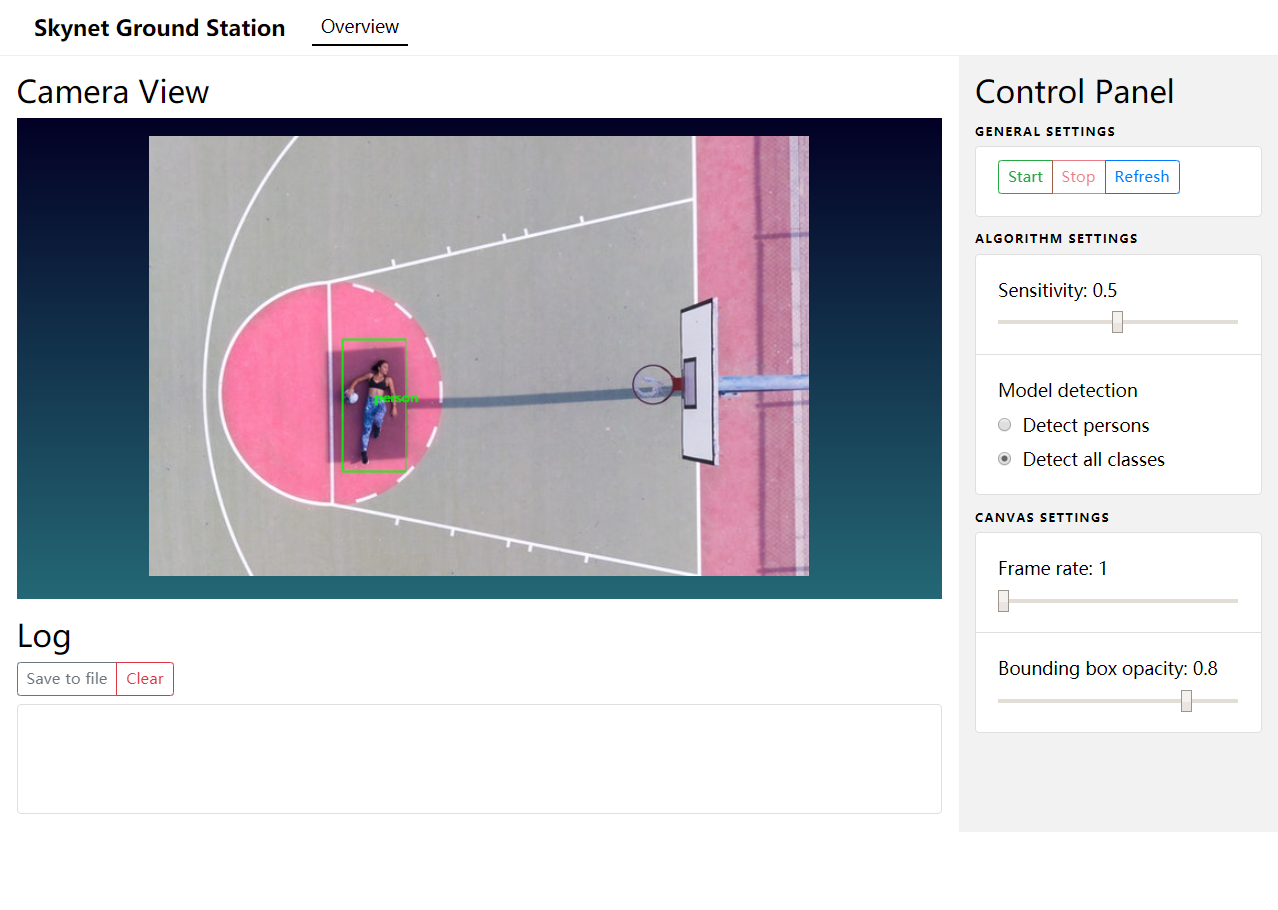
\includegraphics[width=15cm]{img/base_station.png}
\end{mdframed}
\caption{Screen Shot of the Web-app Running on the Base Station}
\label{basestationdiag}
\end{figure}

The Base Station (a Windows/Mac/Linux laptop) hosts a \texttt{Socket.IO} server which simultaneously serves both the PMB and any web clients viewing the results. In doing so, the server continuously queries the PMB for live video data and ML metadata results, and sends the data to the connected web-application clients for display.

The ML results are displayed as a bounding box around the detected object(s) in the frame (\textbf{F.BS.1}) and the type of the object detected is also displayed near the object (see Figure \ref{basestationdiag}). In particular, the ML results consist of three parts: the class of the detected object(s), the coordinates of the upper-left vertex of the bounding box(es), and the height/width of the bounding box(es).

The web application also displays real-time system status messages to the user. These status messages include information on initiation or completion of processes, changes in PMB, PLB or Base Station settings, and system warnings/errors.

In addition, the web application allows the user to adjust several configuration options, including:

\begin{itemize}
\item Enabling/disabling ML processing,
\item Adjusting the ML model's detection sensitivity,
\item Adjusting which classes are reported to the user,
\item Adjusting the frame rate seen by the user, and
\item Adjusting the aesthetics of the ML result overlay
\end{itemize}

\subsubsection{Programming Libraries}

There are two JavaScript libraries used across the client-side and server-side code of the base station:

\texttt{Socket.IO} enables real-time, bidirectional, event-based communication between the browser and the server. We use \texttt{Socket.IO} to facilitate the communication between the base station, its web-app clients, and the PMB. 

\textit{p5.js} is a client-side JavaScript framework that provides programmers with tools to easily generate virtual canvases. We use p5.js to draw the live video feed and ML bounding box data, providing an elegant and high-level approach to convey data to the user.
